\chapter{Introduction and Background} \label{Chap2}
\pagenumbering{arabic}

\section{Introduction}
Quantum computing promises to solve otherwise unsolvable problems. More specifically, problems that would be practically impossible to solve on a classical computer. At the heart of quantum computing lies quantum mechanics, a theory fundamentally different from classical physics. While classical computers encode information in binary digits (bits) that take on definite states of either 0 or 1, quantum computers leverage quantum bits (qubits) which can exist in superpositions of both states simultaneously. This unique property allows quantum computers to explore multiple possibilities concurrently, providing exponential computational advantages for certain classes of problems. Moreover, quantum entanglement, another fundamental quantum phenomenon, enables powerful correlations between qubits that significantly enhance computational efficiency and information processing capabilities. These principles underlie quantum algorithms such as Shor's algorithm for integer factorisation \cite{365700} and Grover's algorithm for unstructured search \cite{10.1145/237814.237866}, each offering dramatic speed-ups over classical counterparts. Additionally, quantum computers are particularly adept at simulating complex quantum systems such as molecules, chemical reactions, or condensed matter phenomena which classical computers handle inefficiently due to exponential resource demands. 

The quantum states underlying these remarkable advantages are inherently fragile. Unlike classical bits, qubits maintain coherence the delicate quantum mechanical property essential for computation only under stringent environmental isolation. Even slight interactions with the external environment, such as thermal fluctuations, electromagnetic radiation, or unintended coupling with neighboring qubits, can quickly degrade quantum coherence. This phenomenon, known as decoherence, rapidly reduces the quantum state from a coherent superposition into a classical probabilistic mixture, thereby erasing quantum advantages and introducing significant errors into computations. Additionally, quantum gates operations used to manipulate quantum states are themselves imperfect. Gate operations introduce systematic errors due to inaccuracies in control signals, calibration imperfections, and hardware limitations, collectively diminishing computational reliability \cite{bultrini2020simplemitigationstrategysystematic}.

Besides improvements to hardware such as enhancing qubit quality, isolation from environmental noise, and precision control of quantum operations, addressing these significant challenges also requires fault-tolerant quantum error correction methods \cite{Calderbank_1996}. Fault tolerance broadly refers to the ability of a quantum computing system to detect, isolate, and correct errors without compromising quantum coherence or the integrity of quantum information \cite{cdi_askewsholts_vlebooks_9780511985249}. Achieving fault tolerance is critical because quantum errors cannot be eliminated entirely due to fundamental physical limitations. By employing carefully designed protocols and optimised quantum circuits, fault-tolerant quantum computing ensures computations can proceed reliably despite the inevitability of errors. Crucially, an essential element of fault-tolerant quantum computing is the efficient design and minimisation of quantum circuits. Minimising quantum circuits reduces exposure to environmental noise, lowers error rates \cite{yu2022analysiserrorpropagationquantum}, and improves overall computational accuracy and scalability.

The necessity to execute quantum algorithms efficiently with the fewest possible operations highlights the importance of circuit optimisation techniques. Efficient circuit implementations are vital to maintain coherence, minimise resource consumption, and maximise the practical utility of quantum computing hardware. Consequently, the central objective of this research is to design a search algorithm specifically tailored to identify the logical implementation of Clifford operations that uses the fewest possible number of two-qubit gates, namely transvections. By designing a metaheuristic search algorithm and selecting optimal logical operator implementations, this project seeks to provide a means to significantly reduce circuit complexity, lower error rates, and improve quantum computational efficiency. Ultimately, this contributes directly to the broader goal of realising robust, scalable, and fault-tolerant quantum computing technologies.

\section{Background}
\subsection{Quantum Error Correction}
As mentioned before, quantum systems are inherently fragile due to the numerous errors arising from interactions with the external environment. Unlike classical information bits, quantum bits (qubits) cannot be copied due to the no-cloning theorem \cite{Wootters1982ASQ}, nor can they be measured without causing the collapse of the quantum state. These constraints make classical redundancy-based error correction challenging to implement. Quantum error correction (QEC) circumvents these limitations by encoding logical quantum information into entangled states across multiple physical qubits, leveraging quantum entanglement and superposition to distribute the information of a single logical qubit. This encoding process protects logical qubits against errors, including bit flips, phase flips, and decoherence-induced errors.

The general structure of error correction is a two-step process: error detection and recovery \cite{cdi_askewsholts_vlebooks_9780511985249}. During error detection, the quantum state undergoes syndrome measurements that identify whether an error has occurred without directly observing the quantum information itself, thereby preserving coherence. The measured syndrome does not reveal the quantum information stored but rather indicates the specific type and location of errors within the encoded quantum state. In the recovery step, this information guides the application of corrective operations that reverse the detected errors, restoring the quantum state to its intended logical form. Through this careful combination of detection and corrective actions, QEC can help to maintain computational reliability and facilitate scalable, fault-tolerant quantum computing.

\begin{figure}[h]
    \centering
    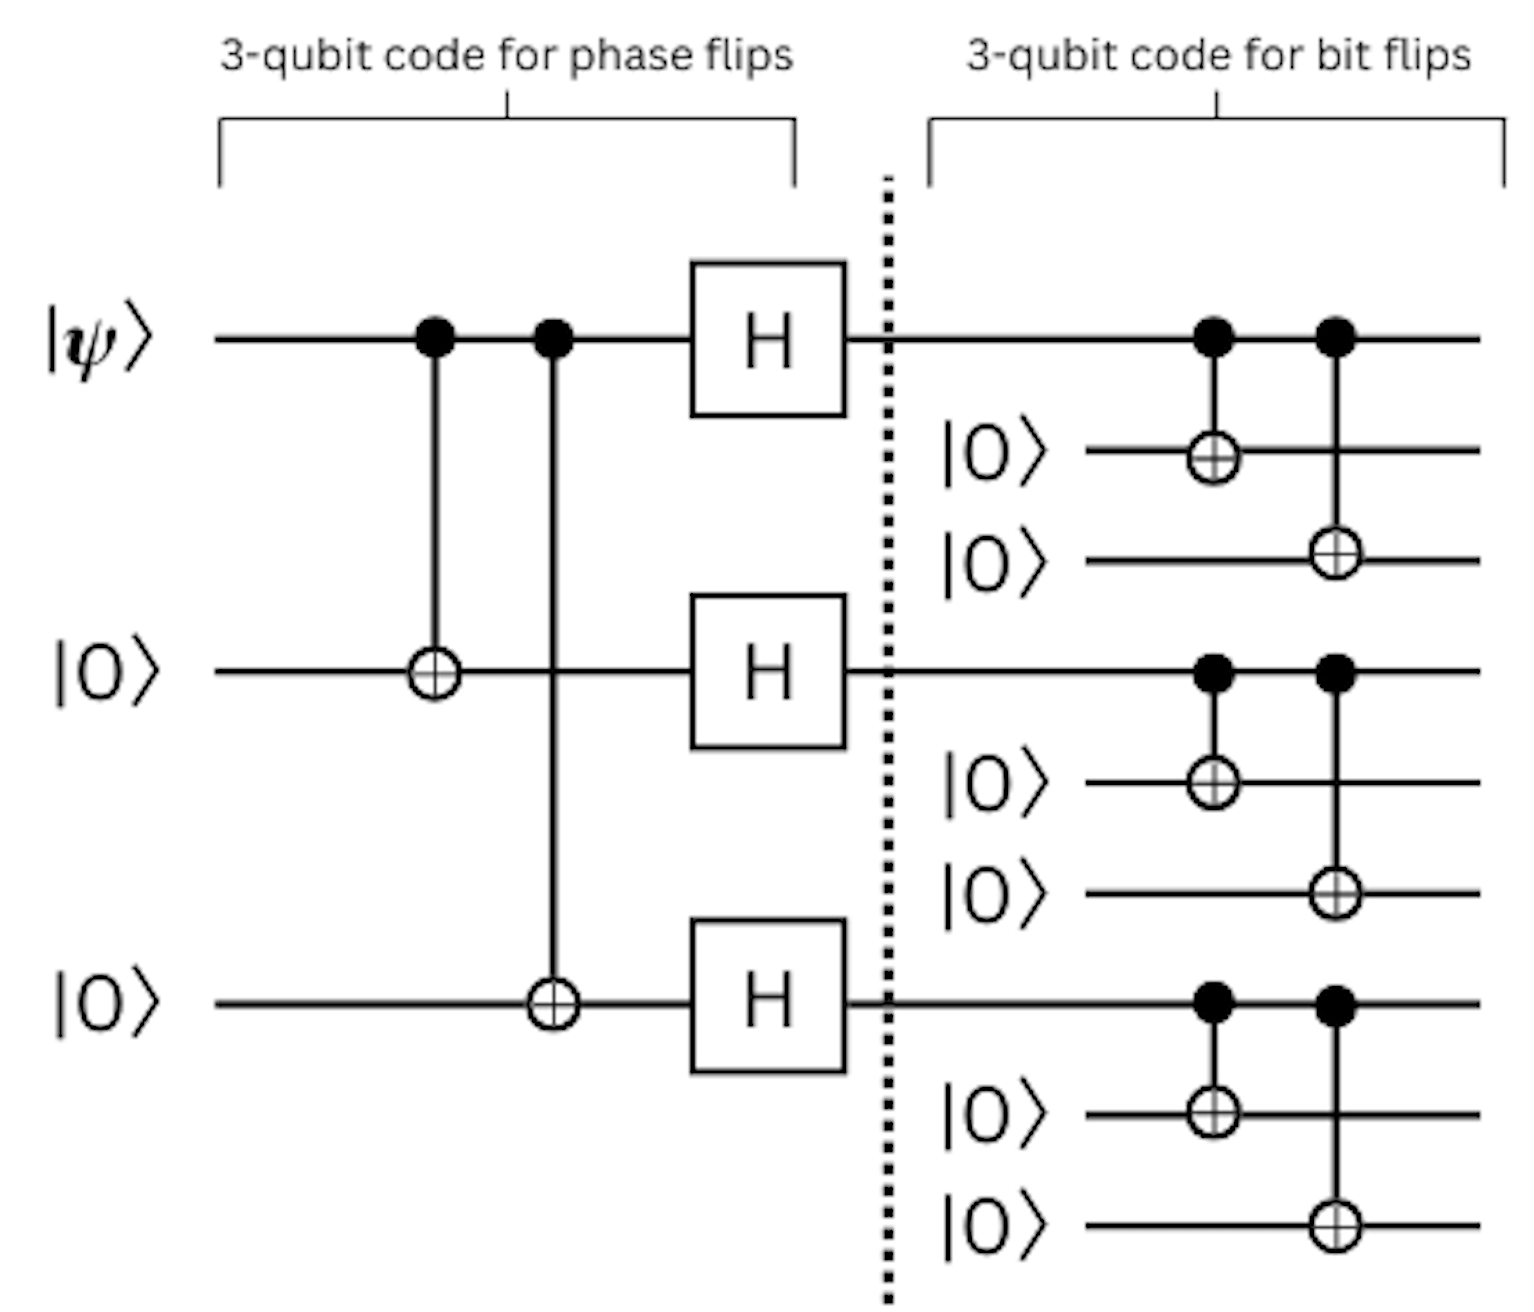
\includegraphics[width=0.5\linewidth]{Logos/Screenshot 2025-03-26 at 21.37.08.png}
    \caption{Circuit diagram of the [[9,1,3]] Shor Code}
    \label{fig:Shor Code Circuit}
\end{figure}

One famous example of an error correction code is the [[9,1,3]] Shor code \cite{PhysRevA.52.R2493} illustrated in Figure \ref{fig:Shor Code Circuit}. The Shor code encodes one logical qubit into nine physical qubits (see equation \ref{eq:logical states}) and is capable of detecting arbitrary two-qubit errors and correcting any single-qubit error. It achieves this by combining two simpler quantum codes: the 3-qubit bit-flip code and the 3-qubit phase-flip code. 

The bit-flip code protects against \(X\) errors, which flip the state of a qubit from |\(0\rangle\) to |\(1\rangle\) or vice versa. It works by encoding a logical qubit into three physical qubits as:

\begin{equation}
    |0_L\rangle=|000\rangle, \quad|1_L\rangle=|111\rangle
\end{equation}

A single bit-flip can be detected by checking parity between qubit pairs and corrected by flipping the erroneous qubit.

The phase-flip code works similarly in the Hadamard basis to protect against \(Z\) errors by detecting phase mismatches. It encodes the logical qubit as:

\begin{equation}
    |0_L\rangle=|+++\rangle, \quad|1_L\rangle=|---\rangle
\end{equation}

where,

\begin{equation}
    |\pm\rangle=\frac{1}{\sqrt{2}}(|0\rangle\pm|1\rangle
\end{equation}

The Shor code concatenates these two codes: it first encodes a logical qubit using the phase-flip code across three blocks, then applies the bit-flip code within each block of three qubits, resulting in the following encoded state:

\begin{equation}
\label{eq:logical states}
    |\psi\rangle = \alpha|0\rangle + \beta|1\rangle \rightarrow |\psi_L\rangle = \alpha|0_L\rangle + \beta|1_L\rangle
\end{equation}

where,

\begin{equation}
    |0_L\rangle=\frac{1}{\sqrt{8}}(|000\rangle+|111\rangle)\otimes(|000\rangle+|111\rangle)\otimes(|000\rangle+|111\rangle)
\end{equation}

and,

\begin{equation}
    |1_L\rangle=\frac{1}{\sqrt{8}}(|000\rangle-|111\rangle)\otimes(|000\rangle-|111\rangle)\otimes(|000\rangle-|111\rangle)
\end{equation}

The layered structure allows the Shor code to detect and correct any single-qubit error bit-flip, phase-flip, or both by measuring stabilisers that reflect parity and phase relationships without collapsing the encoded quantum information. This layered structure allows the Shor code to address both major types of quantum noise, making it a powerful demonstration of how quantum information can be preserved through entanglement and redundancy. Despite its conceptual simplicity, the Shor code captures many of the essential ideas behind more advanced quantum error-correcting codes used in practice today.

\subsection{Stabiliser Formalism}
Stabiliser codes are among the most widely used quantum error correction methods, built upon the mathematical framework of stabiliser formalism. In this approach, quantum states are described by sets of commuting Pauli operators, called stabilisers, which leave the encoded state invariant. Specifically, a unitary operator \(U\) stabilises a state |\(\psi\rangle\) if ,
\begin{equation}
    U|\psi\rangle=|\psi\rangle
\end{equation}
These stabilisers are typically expressed as tensor products of single qubit Pauli operators \(X, Y\), and \(Z\), which satisfy the relations, \(X^2=Y^2=Z^2=I\) and and specific rules outlined in Table \ref{tab:pauli relations}.

\begin{table}[h]
\label{}
\centering
\[
\begin{array}{c|ccc}
 & X & Y & Z \\
\hline
X & 0 & iZ & -iY \\
Y & -iZ & 0 & iX \\
Z & iY & -iX & 0 \\
\end{array}
\]
\caption{Relations of the Pauli operators (entry shows the value of the row times the column).}
\label{tab:pauli relations}
\end{table}

Set of equations defining the actions of \(X, Y\), and \(Z\).

\begin{equation}    
\label{eq:actions of pauli operators}
\begin{aligned}
X \ket{0} &= \ket{1}, & \quad X \ket{1} &= \ket{0} \\
Y \ket{0} &= i\ket{1}, & \quad Y \ket{1} &= -i\ket{0} \\
Z \ket{0} &= \ket{0}, & \quad Z \ket{1} &= -\ket{1}
\end{aligned}
\end{equation}

Using these properties we can demonstrate stabiliser formalism. As an example consider the Bell state,

\begin{equation}
    |\Phi^+\rangle = \frac{\ket{00}+\ket{11}}{\sqrt{2}}
\end{equation}

It is easy to verify that the Pauli operators \(Z_1Z_2\), \(X_1X_2\) and their product, \(-Y_1Y_2\), stabilise |\(\Phi^+\rangle\), since applying all three Pauli operators leaves the state unchanged. Together, these Pauli operators form the stabiliser group of |\(\Phi^+\rangle\), which consists of all operators under which the state remains invariant. An essential property of any stabiliser group is that all its members mutually commute, ensuring that they share a common set of eigenstates. The set of all such shared +1 eigenstates defines the code space, a subspace of the full Hilbert space in which the logical quantum information is encoded and protected. For single state stabiliser codes like |\(\Phi^+\rangle\), this code space is one-dimensional and uniquely determined by the stabiliser group.

Rather than listing the entire stabiliser group, it is often more efficient to describe the state using a stabiliser generator group, a minimal set of independent stabilisers whose combinations generate the full group. In the case of |\(\Phi^+\rangle\), the stabiliser generator group, denoted by \(\langle S\rangle\), is simply \(Z_1Z_2\) and \(X_1X_2\). It turns out that for many QEC codes, stabiliser formalism allows for a more compact and efficient way of representing states as opposed to the typical vector amplitude representation. In particular, quantum circuits composed entirely of Clifford gates such as CNOT, Hadamard, and phase gates are especially well suited to this framework, as these gates preserve the stabiliser structure under conjugation and allow for efficient classical simulation \cite{Aaronson_2004}.

Building on the utility of stabiliser generators, a convenient and compact way to represent them is through the check matrix (also known as the stabiliser tableau). This is a binary matrix of dimensions \(|\langle S \rangle | \times 2n\), where \(n\) is the number of qubits and \(|\langle S \rangle |\) is the number of stabiliser generators. Each row corresponds to one generator, with the first \(n\) columns encoding the presence of \(X\) operators on each qubit and the last \(n\) columns encoding the presence of \(Z\) operators. The presence of a \(Y\) operator is indicated by a 1 in both the \(X\) and \(Z\) components for that qubit. This binary representation greatly simplifies the manipulation and simulation of stabiliser codes, particularly for circuits composed of Clifford operations. It is important to note that the check matrix captures the structure of the generators up to a global phase, which has no effect on the error detecting or error correcting capabilities of the code \cite{webster2024engineeringquantumerrorcorrection}. Despite abstracting away these phases, the check matrix formalism maintains all the essential information needed for error detection and recovery, while remaining computationally efficient and scalable. As an example, the previously discussed \([[9,1,3]]\) Shor code encodes one logical qubit into nine physical qubits and protects against single-qubit errors through combined bit-flip and phase-flip correction, as reflected in its stabiliser generators below.

\begin{table}[h]
\centering
\begin{tabular}{c l}
\toprule
\textbf{Stabilisers } & \textbf{Operator (X, Z)} \\
\midrule
\(S_1\) & \( X_1 X_2 X_3 X_4 X_5 X_6 \) \\
\(S_2\) & \( X_4 X_5 X_6 X_7 X_8 X_9 \) \\
\(S_3\) & \( Z_1 Z_2 \) \\
\(S_4\) & \( Z_2 Z_3 \) \\
\(S_5\) & \( Z_4 Z_5 \) \\
\(S_6\) & \( Z_5 Z_6 \) \\
\(S_7\) & \( Z_7 Z_8 \) \\
\(S_8\) & \( Z_8 Z_9 \) \\
\bottomrule
\end{tabular}
\caption{Stabiliser Generators for the [[9,1,3]] Shor Code.}
\label{tab:shor code generators}
\end{table}

In check matrix form we can represent this code as,

\begin{equation}
\label{eq:shor code check matrix}
\begin{bmatrix}
1 & 1 & 1 & 1 & 1 & 1 & 0 & 0 & 0 \; &\; 0 & 0 & 0 & 0 & 0 & 0 & 0 & 0 & 0 \\
0 & 0 & 0 & 1 & 1 & 1 & 1 & 1 & 1 \; &\; 0 & 0 & 0 & 0 & 0 & 0 & 0 & 0 & 0 \\
0 & 0 & 0 & 0 & 0 & 0 & 0 & 0 & 0 \; &\; 1 & 1 & 0 & 0 & 0 & 0 & 0 & 0 & 0 \\
0 & 0 & 0 & 0 & 0 & 0 & 0 & 0 & 0 \; &\; 0 & 1 & 1 & 0 & 0 & 0 & 0 & 0 & 0 \\
0 & 0 & 0 & 0 & 0 & 0 & 0 & 0 & 0 \; &\; 0 & 0 & 0 & 1 & 1 & 0 & 0 & 0 & 0 \\
0 & 0 & 0 & 0 & 0 & 0 & 0 & 0 & 0 \; &\; 0 & 0 & 0 & 0 & 1 & 1 & 0 & 0 & 0 \\
0 & 0 & 0 & 0 & 0 & 0 & 0 & 0 & 0 \; &\; 0 & 0 & 0 & 0 & 0 & 0 & 1 & 1 & 0 \\
0 & 0 & 0 & 0 & 0 & 0 & 0 & 0 & 0 \; &\; 0 & 0 & 0 & 0 & 0 & 0 & 0 & 1 & 1 \\
\end{bmatrix}
\end{equation}

Expressing a code in check matrix form enables efficient manipulation using binary linear algebra over \(\mathbb{F}_2\) \cite{webster2024engineeringquantumerrorcorrection}. Pauli operators (up to global phase) can be treated as binary vectors, allowing operations like Gaussian elimination to identify independent stabiliser generators. Row additions correspond to multiplying stabilisers, while column operations reflect Clifford conjugation or qubit relabelling. These transformations preserve the code structure, making the check matrix a compact and powerful tool for analysing and evolving stabiliser codes.

\subsection{Logical Operators}
Building on the structure defined by the stabiliser group, a complete description of a stabiliser code also requires specifying the logical operators. While the stabiliser group defines the code space as the simultaneous +1 eigenspace of its generators, logical operators act within this space to manipulate the encoded quantum information. These are Pauli operators that commute with all elements of the stabiliser group ensuring they preserve the code space but are not themselves part of the stabiliser group. This distinction allows them to act non-trivially on the encoded logical qubits. Importantly, because the Pauli group can be represented as a vector space over \( \mathbb{F}_2 \), logical operators can also be expressed and manipulated within the check matrix framework. Identifying logical operators thus becomes an extension of the same algebraic techniques used for analysing stabilisers. These operators are essential for performing computation on encoded qubits, enabling operations such as logical \(X\), \(Z\), or even Clifford gates to be applied directly to encoded data without requiring decoding.

As an example we will look at the [[9,1,3]] code shown in Table \ref{tab:shor code generators}. Here I will simply provide the logical operators for \(X\) and \(Z\), denoted as \(\overline{X}\) and \(\overline{Z}\), to demonstrate their action on the stabiliser group as the method for their construction has been well documented (see papers \cite{webster2024engineeringquantumerrorcorrection} \cite{cdi_askewsholts_vlebooks_9780511985249} for full detail on the construction of Logical \(X\) and \(Z\) from check matrix). The logical \(X\) and \(Z\) are defined as

\begin{equation}
    \overline{X}=Z_1Z_4Z_7, \quad \overline{Z}=X_1X_2X_3
\end{equation}

These operators are not part of the stabiliser group, as they are neither among the generators nor expressible as products of them. However, they commute with all elements of the stabiliser group, ensuring they preserve the code space, and they act non-trivially within it. Like their single-qubit Pauli analogues \(\overline{X}\) and \(\overline{Z}\), consistent with the canonical Pauli relations (see Table \ref{tab:pauli relations}). Moreover, when applied to the encoded logical states of the Shor code (see Equation \ref{eq:logical states}), these logical operators reproduce the standard Pauli actions (see Equation \ref{eq:actions of pauli operators}). These properties confirm that \(\overline{X}\) and \(\overline{Z}\) faithfully implement logical operations on the encoded qubit, just as \(X\) and \(Z\) do in the unencoded single-qubit case.

\subsection{The Clifford Group}
In the context of stabiliser codes, applying arbitrary unitary operations to encoded quantum states can pose a serious problem. Ideally, operations performed on encoded qubits should preserve the structure of the stabiliser group, ensuring that the resulting state remains within the protected code space. However, generic unitary gates can map Pauli operators to non-Pauli operators under conjugation, thereby disrupting the stabiliser structure and potentially introducing undetectable errors. This breaks the assumptions of the stabiliser formalism, which relies on all stabilisers being elements of the Pauli group.

To address this issue, quantum error correction restricts operations to a special subset of unitary gates known as the Clifford group. The Clifford group is defined as the set of unitaries, \(U\), that map Pauli operators, \(M\), to other Pauli operators, \(M'\), under conjugation \cite{gottesman2016surviving} i.e.

\begin{equation}
    UMU^{\dagger}=M'
\end{equation}

This property guarantees that the transformed stabiliser group remains entirely within the Pauli group, preserving error detectability and compatibility with syndrome measurement. The Clifford group includes gates such as the Hadamard (H), Phase (S), and controlled-NOT (CNOT), all of which are foundational to quantum error correction and fault-tolerant quantum computation, however they are not universal for quantum computation.

A key feature of the Clifford group is its homomorphism to the binary symplectic group, meaning that Clifford gates can be represented as binary symplectic matrices. A binary symplectic matrix is a \(2n\times2n\) matrix over \(\mathbb{F}_2 \) that preserves the symplectic inner product \cite{rengaswamy2018synthesis}, a bilinear form that encodes the commutation relationships of Pauli operators. Specifically, a matrix \(M\) is symplectic if it satisfies:

\begin{equation}
\label{eq:symplectic matric property}
    M^T\Omega M=\Omega,
\end{equation}
where,
\begin{equation}
    \Omega = 
    \begin{bmatrix}
    0 & I_n \\
    I_n & 0 \\
    \end{bmatrix}
\end{equation}

This condition ensures that conjugation by a Clifford gate preserves the commutation and anti-commutation structure of Pauli operators. The symplectic representation enables the use of efficient classical algorithms to simulate and manipulate Clifford operations without requiring full complex-valued unitary matrices. For instance, each Clifford gate can be mapped to a symplectic matrix that reflects how it transforms Pauli operators under conjugation. The Hadamard gate, for example, swaps \(X\) and \(Z\) under conjugation, and is represented by the symplectic matrix:

\begin{equation}
H=
\begin{bmatrix}
    0 & 1 \\
    1 & 0 \\
\end{bmatrix}
,
\end{equation}

where the first row corresponds to where \(X\) is mapped to,  and the second row corresponds to where \(Z\) is mapped to. Specifically, under conjugation by the Hadamard gate, \(X\rightarrow Z\) and \(Z\rightarrow X\). This action is reflected in the matrix, the \(X\) component (first column) is swapped with the \(Z\) component (second column). We can also easily verify H upholds Equation \ref{eq:symplectic matric property}, confirming that it preserves the symplectic inner product and thus maintains the commutation relations between Pauli operators under conjugation.

Another powerful feature of the stabiliser formalism is its ability to track the evolution of stabiliser codes under Clifford operations using the tableau representation(see paper Engineering quantum error correction codes using
evolutionary algorithms \cite{webster2024engineeringquantumerrorcorrection} for complete description):

\begin{equation}
    \tau=
    \begin{bmatrix}
        S_x \\
        S_z \\
        L_z \\
        R_x \\
        R_z \\
        L_x
    \end{bmatrix},
\end{equation}

where,

\begin{equation}
    \begin{bmatrix}
        R_x\\
        R_z
    \end{bmatrix}
    =
    \begin{bmatrix}
        0&0&0&I&0&0\\
        0&I&0&0&0&0
    \end{bmatrix}
\end{equation}

In this structure, \(S_x\) and \(S_z\) represent the \(X\) and \(Z\) components of the stabiliser generators that define the code space. The rows \(L_x\) and \(L_z\) correspond to the logical Pauli operators (previously denoted as \(\overline{X}\) and \(\overline{Z}\)) that act non-trivially on the encoded qubits while preserving the stabiliser group. The remaining rows, \(R_x\) and \(R_z\), are known as the destabilisers, which form part of a full operator basis and are essential for decoding and syndrome analysis. Together, these blocks of the tableau encode the full algebraic structure of the stabiliser code and support efficient classical simulation \cite{Aaronson_2004}, encoding transformations, and the implementation of logical operations within the Clifford framework.
The tableau format encodes the stabiliser generators, logical operators, and destabilisers as binary symplectic matrices, enabling compact and efficient simulation of quantum error correcting codes. This structure preserves the symplectic inner product and thus the commutation relationships among Pauli operators, even as Clifford operations transform them.

The tableau representation is particularly useful because it not only compactly captures the structure of stabiliser codes but also acts as an encoding operator. It maps an initial quantum state, consisting of \(k\) logical qubits and \(n-k\) ancillary qubits, into an encoded state within the stabilised code space of \(n\) physical qubits. This transformation is expressed by the following mapping:

\begin{equation}
\begin{large}
\begin{tikzcd}
\mathcal{H}_2^{n-k} \otimes \mathcal{H}_2^k \arrow[r, "\mathcal{\tau}"]  &
\mathcal{H}_2^n
\end{tikzcd}
\end{large}
\end{equation}

Here, \(\mathcal{H}_2^k\)  represents the Hilbert space of the \(k\) logical qubits containing the input quantum information, while \(\mathcal{H}_2^{n-k} \) represents the ancillary qubits initialised in known basis states (typically \(|0\rangle\)). Specifically, given a Clifford operator associated with a binary symplectic matrix \(\tau\), the tableau allows us to construct an encoding circuit that implements the transformation |\(\psi\rangle \rightarrow |\overline{\psi}\rangle\), embedding logical qubits into a protected subspace.

Clifford operations can also be composed using (symplectic) transvections, a type of symplectic transformation that acts minimally on the qubit register and is particularly useful for reducing the number of two-qubit gates. Since two-qubit gates are typically more error-prone than single-qubit gates due to the complex interactions and control precision required for entangling operations between qubits \cite{maldonado2022error}, minimising their use is crucial for building robust and fault-tolerant quantum circuits. Expressing Clifford circuits as sequences of transvections provides an efficient way to reduce circuit depth and control error propagation.

A symplectic transvection is a special kind of operator 

\begin{equation}
\label{eq:transvection definition}
    T_v=I+\Omega v^Tv
\end{equation}

where \(v\in \mathbb{F}_2^{2n} \) \cite{volanto2023minimizing}. In the Clifford domain, they correspond to operations that conjugate Pauli operators in a structured way and can be interpreted as square roots of Pauli matrices. Importantly, any Clifford operator can be decomposed into a product of at most \(2n\) such transvections, meaning they form a universal generating set for the symplectic group. Specific Clifford gates also have simple transvection decompositions, for example a CNOT gate can be written as a product of three transvections:

\begin{equation}
    CNOT_{i,j}=T_{[e_j,0]}T_{[e_j,e_i]}T_{[0,e_i]}
\end{equation}

This decomposition framework makes transvections a powerful tool for designing low-depth Clifford circuits with minimal two-qubit gate usage, as explored in \cite{volanto2023minimizing}.


\section{Project Aim}
While not universal for quantum computation, the Clifford group underpins most quantum error correction schemes by enabling fast, fault-tolerant logical gate implementations that preserve stabiliser structures. Any logical Clifford operator can be decomposed into transvections, SWAPs, and single-qubit Cliffords, with transvections, requiring error-prone two-qubit gates, being the most costly \cite{volanto2023minimizing}. This project develops a search algorithm to minimise transvections in such decompositions, thereby enhancing the efficiency and fault-tolerance of stabiliser code implementations for scalable quantum computing.